\documentclass[a4paper,12pt]{article}
\usepackage[utf8]{inputenc}
\usepackage{graphicx}
\usepackage{amsmath}
\usepackage{hyperref}
\usepackage{geometry}
\usepackage{xcolor}
\usepackage{listings}
\usepackage{newunicodechar}
\usepackage{times}
\geometry{margin=1in}

\newunicodechar{│}{\textbar}

\title{Actuarial Climate Index Documentation}
\author{KANE Dabakh}
\date{July 23rd, 2024}

% Custom settings for listings with more muted colors
\lstset{
    basicstyle=\ttfamily\footnotesize,
    keywordstyle=\color{blue!60!black},
    stringstyle=\color{brown},
    commentstyle=\color{olive},
    backgroundcolor=\color{gray!5},
    frame=single,
    showstringspaces=false,
    breaklines=true,
    postbreak=\mbox{\textcolor{red}{$\hookrightarrow$}\space},
    captionpos=b,
    tabsize=4,
    numbers=left,
    numberstyle=\tiny\color{gray},
    numbersep=10pt,
    language=Python,
    xleftmargin=15pt,
}

\begin{document}

\maketitle

\tableofcontents
\newpage

\section{Introduction}
\label{sec:introduction}

Climate change represents an increasingly significant challenge for modern societies, affecting not only the natural environment but also infrastructures, the economy, and the quality of life. Among the many manifestations of climate change are rising average temperatures, intensifying extreme weather events such as floods, droughts, and storms, as well as rising sea levels. These transformations have direct consequences on various sectors, including agriculture, water management, energy, and, crucially, the insurance industry.

In response to these challenges, actuaries play a crucial role in assessing climate risks and developing appropriate management strategies. It is in this context that the Actuaries Climate Index™ (ACI) was developed—a tool designed to measure changes in climate extremes over time, particularly in the United States and Canada. The ACI provides an objective and quantifiable measure of climate risks, enabling actuaries, policymakers, and the general public to better understand climate trends and adopt suitable measures.

The ACI is based on the analysis of several key climate variables, such as temperature, precipitation, wind speed, and sea level. These variables are integrated into a mathematical model that calculates anomalies relative to a defined reference period. The result is a composite index reflecting the intensity of climate extremes in a given region. By providing a robust and transparent tool for climate risk assessment, the ACI helps strengthen societal resilience to the impacts of climate change.

This document provides a detailed description of the components of the ACI, as well as the methods used to calculate and interpret the index. We also explore the technical aspects related to the implementation of the model, focusing on the use of climate data, the calculation of anomalies, and the standardization of results.

\section{Installation}
\label{sec:installation}

To ensure the proper functionality of the Actuaries Climate Index™ (ACI) project, it is essential to set up a compatible Python environment with the necessary dependencies. Given the specific versions of some packages required by the project, particularly due to compatibility issues between recent versions of \texttt{xarray} and \texttt{numpy}, we recommend using \texttt{conda} to create a dedicated environment for the project. This environment will isolate the dependencies and prevent conflicts with other projects.

\subsection{Steps to Install the ACI Project}
\subsubsection{Install Miniconda or Anaconda}
If you haven't already installed Miniconda or Anaconda, you can download and install one of them from the following links:
\begin{itemize}
    \item \href{https://docs.conda.io/en/latest/miniconda.html}{Miniconda}
    \item \href{https://www.anaconda.com/products/distribution}{Anaconda}
\end{itemize}
Follow the instructions on the website to complete the installation on your operating system.

\subsubsection{Create a New Conda Environment}
Open a terminal or command prompt and run the following command to create a new conda environment specifically for the ACI project. This environment will use Python 3.9, as it is the version compatible with the required packages:

\begin{lstlisting}[language=bash]
conda create --name aci python=3.9
\end{lstlisting}

After the environment is created, activate it with:

\begin{lstlisting}[language=bash]
conda activate aci
\end{lstlisting}

\subsubsection{Install the Required Dependencies}
With the environment activated, install the necessary packages using the \texttt{conda} package manager. The environment file below lists all the dependencies:

\begin{lstlisting}[language=bash]
    name: aci_env
    channels:
      - conda-forge
      - defaults
    dependencies:
      - xarray
      - bottleneck
      - requests
      - netCDF4
      - dask
      - psutil
      - pandas
\end{lstlisting}

To install the packages, you can either copy the content above into a file named \texttt{environment.yml} and run:

\begin{lstlisting}[language=bash]
conda env create -f environment.yml
\end{lstlisting}

Or, manually install each package using the following command:

\begin{lstlisting}[language=bash]
    conda install -c conda-forge xarray bottleneck requests netCDF4 dask psutil pandas
\end{lstlisting}

\subsubsection{Verify the Installation}
After installation, verify that the packages are correctly installed by running Python and importing the necessary libraries:

\begin{lstlisting}[language=bash]
python
\end{lstlisting}

Inside the Python interpreter, try importing the libraries:

\begin{lstlisting}[language=python]
import numpy as np
import xarray as xr
import matplotlib.pyplot as plt
\end{lstlisting}

If no errors occur, your environment is correctly set up.

\subsubsection{Run Jupyter Notebook (Optional)}
If you plan to use Jupyter Notebook for working with the project, you can start it by running:

\begin{lstlisting}[language=bash]
jupyter notebook
\end{lstlisting}

This command will open a Jupyter Notebook interface in your web browser, allowing you to interactively work with the ACI project.

\subsection{Important Notes}
\begin{itemize}
    \item \textbf{Compatibility:} This setup ensures that you avoid known compatibility issues between \texttt{xarray} and \texttt{numpy}. The specified versions are critical for the proper functioning of the ACI project.
    \item \textbf{Environment Isolation:} Using a \texttt{conda} environment ensures that the installed packages do not interfere with other Python projects on your system. It also makes it easier to manage dependencies specific to the ACI project.
\end{itemize}

\section{Project Structure}
\label{sec:structure}

The Actuaries Climate Index™ (ACI) project is organized into several directories and files, each serving a specific purpose in the development, execution, and maintenance of the project. This structure is designed to separate the source code, data, documentation, and tests, facilitating collaborative development and efficient maintenance.

\subsection{Root Directory}

The root directory of the ACI project contains the following key components:

\begin{itemize}
    \item \textbf{aci/}: This directory contains the core Python scripts and modules essential for calculating the Actuaries Climate Index™. The scripts here handle data processing, integration of various climate components, and the computation of the index.
    \begin{itemize}
        \item \textbf{aci.py}: The central script that coordinates the integration of different components to calculate the ACI.
        \item \textbf{components/}: A subdirectory that houses modular Python scripts, each dedicated to handling a specific climate variable such as temperature, precipitation, wind, and sea level.
        \item \textbf{request\_copernicus\_data.py} and \textbf{request\_sealevel\_data.py}: These scripts are responsible for downloading and processing climate data from external sources like the Copernicus Climate Data Store and sea level databases.
    \end{itemize}
    \item \textbf{data/}: This directory stores all data files used by the project, structured into subdirectories to organize the raw input data and required data files for processing.
    \begin{itemize}
        \item \textbf{required\_data/}: Contains essential data files necessary for the project's operations, including NetCDF files for various climate variables and gridded country data.
        \item \textbf{tests\_data/}: This subdirectory holds test data that mimics the structure of the actual data but on a smaller scale, used for testing the project's components.
    \end{itemize}
    \item \textbf{documentation/}: This directory contains the LaTeX source files needed to generate the project's documentation, as well as the compiled PDF and auxiliary files.
    \item \textbf{tests/}: The tests directory includes all unit tests for the project’s various components. Each Python file here is dedicated to testing a specific module, ensuring the correctness of the implementation.
    \item \textbf{README.md}: A markdown file providing an overview of the project, along with basic instructions on how to set up and use the ACI project.
    \item \textbf{environment.yml}: A YAML file listing all the dependencies required to run the project, intended for use with conda to set up a compatible environment.
    \item \textbf{requirements.txt}: Similar to \texttt{environment.yml}, this file lists the Python packages required for the project, typically used for setting up a virtual environment with \texttt{pip}.
    \item \textbf{setup.py}: A script for setting up the project as a Python package, facilitating its installation and deployment.
\end{itemize}

\subsection{aci/ Directory}
The \textbf{aci/} directory is the core of the project, containing the main script (\texttt{aci.py}) that integrates the various components to compute the Actuaries Climate Index™. Within this directory, the \textbf{components/} subdirectory holds modular scripts for handling different climate variables. For instance:

\begin{itemize}
    \item \textbf{aci.py}: Acts as the central hub for processing and integrating data from all components to generate the ACI.
    \item \textbf{components/}: A collection of scripts, each dedicated to a specific climate variable. These include:
    \begin{itemize}
        \item \textbf{component.py}: The base class from which all other components inherit.
        \item \textbf{drought.py}: Manages data related to drought conditions.
        \item \textbf{precipitation.py}: Handles precipitation data processing.
        \item \textbf{sealevel.py}: Manages sea level data and processing.
        \item \textbf{temperature.py}: Processes temperature data.
        \item \textbf{wind.py}: Deals with wind data, including wind power calculations.
    \end{itemize}
    \item \textbf{request\_copernicus\_data.py} and \textbf{request\_sealevel\_data.py}: These scripts are used for downloading and processing data from external sources such as Copernicus Climate Data Store and sea level databases, ensuring the project has up-to-date climate data.
\end{itemize}

\subsection{components/ Directory}
The \textbf{components/} directory is crucial as it houses the modular scripts for each climate component. Each script focuses on a different aspect of climate data:

\begin{itemize}
    \item \textbf{component.py}: Serves as the foundational class from which other component classes inherit methods and attributes.
    \item \textbf{drought.py}: Specializes in the processing and analysis of drought data.
    \item \textbf{precipitation.py}: Focuses on handling and analyzing precipitation data.
    \item \textbf{sealevel.py}: Deals with the processing of sea level data.
    \item \textbf{temperature.py}: Manages temperature data, including the calculation of anomalies and extremes.
    \item \textbf{wind.py}: Handles wind data, including calculations related to wind power and thresholds.
\end{itemize}

\subsection{data/ Directory}
The \textbf{data/} directory is dedicated to storing all data files used by the project. This directory is organized into subdirectories for clarity:

\begin{itemize}
    \item \textbf{required\_data/}: This subdirectory contains the critical data files necessary for the project's operations, such as gridded country data and NetCDF files for various climate variables.
    \item \textbf{tests\_data/}: Stores test data that is structured similarly to the actual data but on a smaller scale. This data is used to test the functionality of the project without processing large datasets.
\end{itemize}

\subsection{required\_data/ Directory}
Within the \textbf{required\_data/} directory, essential data files are stored. These include:

\begin{itemize}
    \item \textbf{1960-1970/}: A subdirectory containing NetCDF files for various climate variables (e.g., wind, temperature, precipitation) from 1960 to 1970, which are likely used as sample data for analysis and testing.
    \item \textbf{countries\_gridded\_0.1deg\_v0.1\_FRo.nc}: A NetCDF file containing gridded climate data specific to France.
    \item \textbf{rlr\_monthly/}: This subdirectory contains monthly sea level data from the Permanent Service for Mean Sea Level (PSMSL), including various metadata files necessary for processing the sea level data.
\end{itemize}

\subsection{tests/ Directory}
The \textbf{tests/} directory contains unit tests that are critical for ensuring the functionality and reliability of the project's components. Each test script is dedicated to a specific module:

\begin{itemize}
    \item \textbf{test\_drought.py}: Contains unit tests for the drought component, verifying its correctness.
    \item \textbf{test\_precipitation.py}: Tests the functionality of the precipitation component.
    \item \textbf{test\_sealevel.py}: Ensures that the sea level component processes data correctly.
    \item \textbf{test\_temperature.py}: Contains tests for the temperature component, ensuring accurate data processing.
    \item \textbf{test\_wind.py}: Verifies the calculations related to wind data within the project.
    \item \textbf{test\_aci.py}: Contains tests that validate the overall ACI calculation process, integrating all components.
\end{itemize}

\subsection{Project Directory Structure Diagram}

To provide a visual understanding of the project's organization, below is a diagram representing the directory structure:

\begin{verbatim}
    aci_project/
    |
    +-- aci/
    |   +-- aci.py
    |   +-- components/
    |       +-- component.py
    |       +-- drought.py
    |       +-- precipitation.py
    |       +-- sealevel.py
    |       +-- temperature.py
    |       +-- wind.py
    +-- data/
    |   +-- required_data/
    |   |   +-- 1960-1970/
    |   |   +-- countries_gridded_0.1deg_v0.1_FRo.nc
    |   |   +-- rlr_monthly/
    |   +-- tests_data/
    +-- documentation/
    |   +-- documentation.tex
    |   +-- documentation.pdf
    +-- tests/
    |   +-- test_drought.py
    |   +-- test_precipitation.py
    |   +-- test_sealevel.py
    |   +-- test_temperature.py
    |   +-- test_wind.py
    +-- environment.yml
    +-- requirements.txt
    +-- setup.py
    +-- README.md

\end{verbatim}

\section{Usage}
\label{sec:usage}

This section describes how to use the Actuarial Climate Index™ (ACI) project to perform climate data analyses, download necessary data, and calculate the climate index. The examples provided cover the use of the main components, including data downloading and processing.

\subsection{Downloading Data via the Copernicus API}

To download climate data such as ERA5 data using the Copernicus API, you can use the 'request\_copernicus\_data.py' script. Here’s how to request data:

\begin{lstlisting}[language=python]
from aci.request_copernicus_data import Era5var

# Define the area, coordinates, year range, and variable to download
area = 'France'
coordinates = [51.0, -5.0, 41.0, 9.0]  # North, West, South, East
years = '1980-1981'
variable_name = '2m_temperature'

# Initialize the data request for ERA5
era5 = Era5var(area, coordinates, years, variable_name, monthly=True)

# Request and download the data
era5.request_data()

# The data will be saved in the specified directory as NetCDF files.
\end{lstlisting}

This will download ERA5 data for the specified area and time period, saving it as NetCDF files.

\subsection{Downloading and Processing Sea Level Data}

To download and process sea level data using the Permanent Service for Mean Sea Level (PSMSL) data, use the 'request\_sealevel\_data.py' script as follows:

\begin{lstlisting}[language=python]
from aci.request_sealevel_data import download_and_extract_data, load_dataframe, copy_and_rename_files_by_country

# Download and extract the PSMSL data
download_and_extract_data()

# Load the DataFrame containing metadata about the sea level data
df = load_dataframe()

# Copy and rename files for a specific country (e.g., France)
country_abbrev = 'FRA'
copy_and_rename_files_by_country(country_abbrev, df)

# The sea level data will now be available in the `../data/sealevel_data_FRA/` directory.
\end{lstlisting}

\subsection{Processing Temperature Data}

To process temperature data and calculate temperature-based climate indices:

\begin{lstlisting}[language=python]
from aci.components.temperature import TemperatureComponent

# Example 1: Initialize with a single file and no mask
temperature_component = TemperatureComponent(
    'data/required_data/temperature_1960-1970.nc'
)

# Example 2: Initialize with a directory and an optional mask
temperature_component = TemperatureComponent(
    'data/required_data/temperature_data/', 
    'data/required_data/mask.nc'
)

# Calculate the T90 index (90th percentile exceedance)
t90_values = temperature_component.std_t90(('1961-01-01', '1990-12-31'))

# Calculate the T10 index (10th percentile exceedance)
t10_values = temperature_component.std_t10(('1961-01-01', '1990-12-31'))

print(f"T90 Values: {t90_values}")
print(f"T10 Values: {t10_values}")
\end{lstlisting}

\subsection{Processing Precipitation Data}

To process precipitation data and calculate related indices:

\begin{lstlisting}[language=python]
from aci.components.precipitation import PrecipitationComponent

# Example 1: Initialize with a single file and no mask
precipitation_component = PrecipitationComponent(
    'data/required_data/precipitation_1960-1970.nc'
)

# Example 2: Initialize with a directory and an optional mask
precipitation_component = PrecipitationComponent(
    'data/required_data/precipitation_data/', 
    'data/required_data/mask.nc'
)

# Calculate the anomaly of maximum monthly precipitation
monthly_max_anomaly = precipitation_component.monthly_max_anomaly(
    "tp", 5, ('1961-01-01', '1990-12-31')
)

print(f"Monthly Max Anomaly: {monthly_max_anomaly}")
\end{lstlisting}

\subsection{Processing Wind Data}

To process wind data and calculate wind-related indices:

\begin{lstlisting}[language=python]
from aci.components.wind import WindComponent

# Example 1: Initialize with single files for u10, v10, and no mask
wind_component = WindComponent(
    'data/required_data/wind_u10_1960-1970.nc',
    'data/required_data/wind_v10_1960-1970.nc'
)

# Example 2: Initialize with directories for u10, v10, and an optional mask
wind_component = WindComponent(
    'data/required_data/wind_u10_data/', 
    'data/required_data/wind_v10_data/',
    'data/required_data/mask.nc'
)

# Calculate wind exceedance frequency
wind_exceedance = wind_component.std_wind_exceedance_frequency(('1961-01-01', '1990-12-31'))

print(f"Wind Exceedance Frequency: {wind_exceedance}")
\end{lstlisting}

\subsection{Processing Sea Level Data}

To process sea level data using the SeaLevelComponent:

\begin{lstlisting}[language=python]
from aci.components.sealevel import SeaLevelComponent

# Define study and reference periods
study_period = ('1980-01-01', '2020-12-31')
reference_period = ('1961-01-01', '1990-12-31')

# Initialize the SeaLevelComponent with the country abbreviation and periods
sea_level_component = SeaLevelComponent('FRA', study_period, reference_period)

# Process the sea level data
processed_sea_level_data = sea_level_component.process()

# View the processed sea level data
print(processed_sea_level_data)
\end{lstlisting}

\subsection{Running a Complete Pipeline}

To run a complete pipeline, integrating multiple components and calculating the Actuarial Climate Index:

\begin{lstlisting}[language=python]
from aci.aci import ActuarialClimateIndex

# Example 1: Initialize the Actuarial Climate Index with single file paths and no mask
aci = ActuarialClimateIndex(
    temperature_data_path='data/required_data/temperature_1960-1970.nc',
    precipitation_data_path='data/required_data/precipitation_1960-1970.nc',
    wind_u10_data_path='data/required_data/wind_u10_1960-1970.nc',
    wind_v10_data_path='data/required_data/wind_v10_1960-1970.nc',
    country_abbrev='FRA',
    study_period=('1980-01-01', '2020-12-31'),
    reference_period=('1961-01-01', '1990-12-31')
)

# Example 2: Initialize the Actuarial Climate Index with directories and an optional mask
aci = ActuarialClimateIndex(
    temperature_data_path='data/required_data/temperature_data/', 
    precipitation_data_path='data/required_data/precipitation_data/', 
    wind_u10_data_path='data/required_data/wind_u10_data/',
    wind_v10_data_path='data/required_data/wind_v10_data/',
    country_abbrev='FRA',
    mask_data_path='data/required_data/mask.nc',
    study_period=('1980-01-01', '2020-12-31'),
    reference_period=('1961-01-01', '1990-12-31')
)

# Calculate the overall ACI index
aci_index = aci.calculate_aci()

print(f"Actuarial Climate Index: {aci_index}")
\end{lstlisting}

\subsection{Visualizing the Results}

To visualize the results using Matplotlib:

\begin{lstlisting}[language=python]
import matplotlib.pyplot as plt

# Visualize the T90 index
t90_values.plot()
plt.title("T90 Index (90th Percentile Exceedance)")
plt.show()

# Visualize the Actuarial Climate Index
plt.plot(aci_index['ACI'])
plt.title("Actuarial Climate Index")
plt.xlabel("Time")
plt.ylabel("Index")
plt.show()
\end{lstlisting}

\subsection{Running Unit Tests}

To verify the accuracy of the ACI project, unit tests can be run with the following command:

\begin{lstlisting}[language=bash]
pytest tests/
\end{lstlisting}

This command will execute all tests defined in the `tests/` directory and display the results, confirming whether the different components of the project are functioning correctly.

\section{Components Documentation}
\label{sec:api-documentation-detailed}

\subsection{Component Class}
\label{subsec:component-class}
\textbf{File:} component.py \\
\textbf{Description:} Serves as the base class for various climate data components, providing essential functionalities for data management and parallel processing.

\textbf{Methods:}
\begin{itemize}
    \item \texttt{\_\_init\_\_(self, array, mask, file\_name)}: Constructs the component with specified data and mask arrays. It configures the environment for parallel computation if system resources permit. \\
    \textbf{Parameters:}
    \begin{itemize}
        \item \texttt{array (xarray.Dataset)}: Dataset containing the primary climate data.
        \item \texttt{mask (xarray.Dataset)}: Dataset for masking the data based on geographical or other criteria.
        \item \texttt{file\_name (str)}: Path to the data file.
    \end{itemize}
    \textbf{Complexity:} O(1), as it primarily sets up attributes.
    
    \item \texttt{should\_use\_dask(self)}: Determines whether to utilize Dask for parallel processing by assessing available system resources (CPU and memory). \\
    \textbf{Complexity:} O(1), involves checking system attributes.
    
    \item \texttt{determine\_chunk\_size(self, dataset)}: Calculates optimal chunk sizes for data processing based on available memory, aimed at efficient Dask operation. \\
    \textbf{Parameters:}
    \begin{itemize}
        \item \texttt{dataset (xarray.Dataset)}: The dataset to be chunked for parallel processing.
    \end{itemize}
    \textbf{Complexity:} O(n), where n is the number of dimensions in the dataset as it configures chunking strategy.
    
    \item \texttt{initialize\_dask(self)}: Initializes a Dask client to enable distributed computing, optimizing performance for large data sets. \\
    \textbf{Complexity:} O(1), setup of a Dask cluster based on the system configuration.
    
    \item \texttt{apply\_mask(self, var\_name, threshold=0.8)}: Applies a geographical or conditional mask to the data, which is essential for focusing analysis on specific regions or conditions. \\
    \textbf{Parameters:}
    \begin{itemize}
        \item \texttt{var\_name (str)}: The variable within the dataset to which the mask is applied.
        \item \texttt{threshold (float)}: Threshold value above which data is retained.
    \end{itemize}
    \textbf{Complexity:} O(m), where m is the number of data points in the dataset.
    
    \item \texttt{standardize\_metric(self, metric, reference\_period, area)}: Standardizes a metric using historical data, crucial for trend analysis and anomaly detection in climate studies. \\
    \textbf{Parameters:}
    \begin{itemize}
        \item \texttt{metric (xarray.DataArray)}: The climate metric to standardize.
        \item \texttt{reference\_period (tuple)}: The start and end dates defining the historical period for normalization.
        \item \texttt{area (bool)}: Whether to average the results over a geographical area.
    \end{itemize}
    \textbf{Complexity:} O(p), where p is the number of time steps within the reference period.
    
    \item \texttt{calculate\_rolling\_sum(self, var\_name, window\_size)}: Computes a rolling sum over a specified window size, which is essential for analyzing trends over time. \\
    \textbf{Parameters:}
    \begin{itemize}
        \item \texttt{var\_name (str)}: The variable name to calculate the rolling sum.
        \item \texttt{window\_size (int)}: The number of intervals over which to calculate the sum.
    \end{itemize}
    \textbf{Complexity:} O(q), where q is the number of data points, considering the rolling window size.
\end{itemize}

\subsection{TemperatureComponent Class}
\label{subsec:temperature-component-class}
\textbf{File:} temperature.py \\
\textbf{Description:} Manages temperature data, including the processing of daily extremes and the computation of temperature-based indices such as T90 and T10.

\textbf{Methods:}
\begin{itemize}
    \item \texttt{\_\_init\_\_(self, temperature\_data\_path, mask\_data\_path)}: Initializes the TemperatureComponent with paths to temperature data and a mask. \\
    \textbf{Parameters:}
    \begin{itemize}
        \item \texttt{temperature\_data\_path (str)}: Path to the dataset containing temperature data.
        \item \texttt{mask\_data\_path (str)}: Path to the dataset used for applying geographical masks.
    \end{itemize}
    \textbf{Complexity:} O(1), primarily setup of data paths.

    \item \texttt{temp\_extremum(self, extremum, period)}: Calculates daily minimum or maximum temperatures based on specified time periods (day or night), which is crucial for assessing temperature extremes. \\
    \textbf{Parameters:}
    \begin{itemize}
        \item \texttt{extremum (str)}: Specifies whether to find 'min' or 'max' temperature.
        \item \texttt{period (str)}: Specifies the time period, 'day' or 'night'.
    \end{itemize}
    \textbf{Complexity:} O(r), where r is the number of daily temperature readings in the dataset.

    \item \texttt{percentiles(self, n, reference\_period, tempo)}: Computes percentiles for temperature data, useful for establishing climatological baselines. \\
    \textbf{Parameters:}
    \begin{itemize}
        \item \texttt{n (int)}: The percentile to compute (e.g., 90 for the 90th percentile).
        \item \texttt{reference\_period (tuple)}: The start and end dates for the period over which to calculate percentiles.
        \item \texttt{tempo (str)}: 'day' or 'night' to specify when the percentiles should be calculated.
    \end{itemize}
    \textbf{Complexity:} O(s), where s is the number of data points in the reference period.
\end{itemize}

\subsubsection{PrecipitationComponent Class}
\textbf{File:} precipitation.py

The \texttt{PrecipitationComponent} class extends the \texttt{Component} base class and specializes in processing precipitation data. It offers methods to calculate monthly and seasonal maximum precipitation values and their anomalies. This class is crucial for understanding precipitation trends, which are significant for studying climate change impacts, especially in terms of hydrological extremes such as floods and droughts.

\begin{itemize}
    \item \textbf{Constructor:} \texttt{\_\_init\_\_(self, precipitation\_path, mask\_path)}
    \begin{itemize}
        \item \textbf{Parameters:}
        \begin{itemize}
            \item \texttt{precipitation\_path (str)}: Path to the dataset containing precipitation data.
            \item \texttt{mask\_path (str)}: Path to the dataset containing mask data for filtering the geographic area of interest.
        \end{itemize}
        \item \textbf{Complexity:} O(P), where P is the size of the precipitation dataset. This complexity arises because the method loads the dataset from the file system and initializes the mask.
        \item \textbf{Description:} This constructor initializes the component with the specified datasets, loading the precipitation data and applying a geographical mask if provided. This setup is essential for subsequent calculations that rely on this filtered data.
    \end{itemize}

    \item \textbf{Method:} \texttt{monthly\_max(self, var\_name, window\_size)}
    \begin{itemize}
        \item \textbf{Parameters:}
        \begin{itemize}
            \item \texttt{var\_name (str)}: Variable name in the precipitation dataset to calculate the maximum for.
            \item \texttt{window\_size (int)}: The size of the rolling window in days over which the maximum will be calculated.
        \end{itemize}
        \item \textbf{Complexity:} O(N), where N is the number of time steps in the dataset. This involves rolling window computations which are linear in nature.
        \item \textbf{Returns:} xarray.DataArray containing the maximum precipitation values for each month.
        \item \textbf{Description:} This method calculates the maximum precipitation values over a specified rolling window for each month. This is particularly useful for identifying the most intense precipitation events within each month, which can be critical for flood risk assessment.
    \end{itemize}

    \item \textbf{Method:} \texttt{monthly\_max\_anomaly(self, var\_name, window\_size, reference\_period, area=None)}
    \begin{itemize}
        \item \textbf{Parameters:}
        \begin{itemize}
            \item \texttt{var\_name (str)}: Variable name in the precipitation dataset.
            \item \texttt{window\_size (int)}: Window size in days for calculating maximum precipitation.
            \item \texttt{reference\_period (tuple)}: Start and end dates of the reference period for anomaly calculation.
            \item \texttt{area (bool, optional)}: If provided, calculates the area-averaged anomaly across the specified geographic area.
        \end{itemize}
        \item \textbf{Complexity:} O(N + R), where N is the number of time steps in the dataset and R is the duration of the reference period. The method involves additional complexity due to the standardization process.
        \item \textbf{Returns:} xarray.DataArray of monthly maximum precipitation anomalies.
        \item \textbf{Description:} Calculates anomalies in monthly maximum precipitation relative to a historical baseline defined by the reference period. This method is essential for detecting changes or shifts in precipitation intensity, providing insights into how precipitation extremes are evolving in the context of climate change.
    \end{itemize}
\end{itemize}


\subsubsection{SeaLevelComponent Class}
\textbf{File:} sealevel.py

The \texttt{SeaLevelComponent} is designed to handle sea level data, a critical aspect of climate studies, especially in the context of global warming and its impact on rising sea levels. This class is crucial for analyzing changes in sea levels over time, providing essential data for coastal management and flood risk assessment.

\begin{itemize}
    \item \textbf{Constructor:} \texttt{\_\_init\_\_(self, country\_abbrev, study\_period, reference\_period)}
    \begin{itemize}
        \item \textbf{Parameters:}
        \begin{itemize}
            \item \texttt{country\_abbrev (str)}: Abbreviation of the country for which sea level data is to be analyzed.
            \item \texttt{study\_period (tuple)}: Start and end dates for the period under study.
            \item \texttt{reference\_period (tuple)}: Start and end dates for the historical period used for normalization.
        \end{itemize}
        \item \textbf{Complexity:} Initialization involves setting up the directory structure and preparing the data, but does not involve computational complexity at this stage.
        \item \textbf{Description:} Constructs the necessary attributes for the Sea Level Component, setting up the environment to load, process, and analyze sea level data specific to a given country.
    \end{itemize}

    \item \textbf{Method:} \texttt{load\_data(self)}
    \begin{itemize}
        \item \textbf{Complexity:} O(N * M) where N is the number of files and M is the average number of rows per file. This represents the complexity of reading multiple data files and merging them into a single DataFrame.
        \item \textbf{Returns:} pandas.DataFrame containing concatenated data from all relevant files in the specified directory.
        \item \textbf{Description:} Loads sea level data from files stored in a designated directory, combining them into a comprehensive dataset. This method is essential for preparing the data for further processing and analysis.
    \end{itemize}

    \item \textbf{Method:} \texttt{correct\_date\_format(self, data)}
    \begin{itemize}
        \item \textbf{Parameters:}
        \begin{itemize}
            \item \texttt{data (pd.DataFrame)}: DataFrame containing the original sea level data with dates in float format.
        \end{itemize}
        \item \textbf{Complexity:} O(N), where N is the number of rows in the DataFrame. The complexity arises from converting each date from a float format to a standard date format.
        \item \textbf{Returns:} pandas.DataFrame with corrected date formats.
        \item \textbf{Description:} Converts the date format from a float representation (e.g., 1999.9583 for December 1999) to a standard YYYY-MM-DD format, facilitating easier analysis and visualization of the data.
    \end{itemize}

    \item \textbf{Method:} \texttt{clean\_data(self, data)}
    \begin{itemize}
        \item \textbf{Parameters:}
        \begin{itemize}
            \item \texttt{data (pd.DataFrame)}: DataFrame to be cleaned.
        \end{itemize}
        \item \textbf{Complexity:} O(N), where N represents the number of rows in the DataFrame. This accounts for the operation of replacing sentinel values across the dataset.
        \item \textbf{Returns:} pandas.DataFrame with NaNs replacing any sentinel values that represent missing or erroneous data.
        \item \textbf{Description:} Cleans the dataset by replacing known sentinel values (e.g., -99999) with NaN to prevent them from affecting the subsequent analyses. This is a crucial step to ensure the accuracy of the sea level trends and statistics derived from the data.
    \end{itemize}

    \item \textbf{Method:} \texttt{process(self)}
    \begin{itemize}
        \item \textbf{Complexity:} O(N * M), considering the complexities of loading, cleaning, standardizing, and aggregating data where N is the number of rows and M is the number of processing steps involved.
        \item \textbf{Returns:} pandas.DataFrame that has been fully processed and standardized, ready for detailed analysis or reporting.
        \item \textbf{Description:} Conducts a comprehensive processing of the sea level data which includes loading, date correction, cleaning, and standardizing based on reference periods. This method is essential for preparing the data for in-depth analysis and for generating actionable insights regarding sea level changes.
    \end{itemize}
\end{itemize}



\subsubsection{WindComponent Class}
\textbf{File:} wind.py

The \texttt{WindComponent} class extends the \texttt{Component} base class and specializes in managing and analyzing wind data. It is pivotal for calculating wind power potential and identifying extreme wind events, which are crucial for both energy resource management and risk assessment in storm-prone areas.

\begin{itemize}
    \item \textbf{Constructor:} \texttt{\_\_init\_\_(self, u10\_path, v10\_path, mask\_path)}
    \begin{itemize}
        \item \textbf{Parameters:}
        \begin{itemize}
            \item \texttt{u10\_path (str)}: Path to the dataset containing wind u-component data.
            \item \texttt{v10\_path (str)}: Path to the dataset containing wind v-component data.
            \item \texttt{mask\_path (str)}: Path to the dataset containing mask data for filtering the geographic area of interest.
        \end{itemize}
        \item \textbf{Complexity:} O(W), where W represents the size of the wind dataset. This complexity accounts for loading the datasets from the filesystem and initializing the masks.
        \item \textbf{Description:} This constructor initializes the wind component with the specified datasets for the u and v components of wind, setting the stage for complex vector calculations required for wind power and other analyses.
    \end{itemize}

    \item \textbf{Method:} \texttt{wind\_power(self, reference\_period=None)}
    \begin{itemize}
        \item \textbf{Parameters:}
        \begin{itemize}
            \item \texttt{reference\_period (tuple, optional)}: If provided, calculates daily wind power for the specified reference period, which is crucial for analyzing historical data or specific time frames.
        \end{itemize}
        \item \textbf{Complexity:} O(N) where N is the number of time steps in the dataset. The method involves calculating wind speed from the vector components and then computing the kinetic energy available in the wind.
        \item \textbf{Returns:} xarray.DataArray representing the daily mean wind power, crucial for assessments of wind energy potential.
        \item \textbf{Description:} Calculates daily wind power using the formula \( \frac{1}{2} \rho v^3 \) where \( \rho \) is the air density and \( v \) is the wind speed. This method is integral for determining the energy production capabilities of wind turbines and for assessing potential wind damage during extreme events.
    \end{itemize}

    \item \textbf{Method:} \texttt{wind\_thresholds(self, reference\_period)}
    \begin{itemize}
        \item \textbf{Parameters:}
        \begin{itemize}
            \item \texttt{reference\_period (tuple)}: The start and end dates of the reference period for calculating wind power thresholds.
        \end{itemize}
        \item \textbf{Complexity:} O(N + R) where N is the number of time steps and R is the number of days in the reference period. This includes the complexity of aggregating wind power data and calculating statistical thresholds.
        \item \textbf{Returns:} xarray.DataArray of wind power thresholds based on the 90th percentile, used for categorizing wind events as normal or extreme.
        \item \textbf{Description:} This method establishes thresholds for wind power that categorize days as having normal or extreme wind conditions based on historical data. These thresholds are essential for understanding and predicting storm damage potential and for planning in wind-sensitive industries like insurance and construction.
    \end{itemize}
\end{itemize}


\subsubsection{DroughtComponent Class}
\textbf{File:} drought.py

The \texttt{DroughtComponent} class extends the \texttt{Component} base class and is specifically designed to manage and analyze data related to drought conditions. This class is pivotal for assessing the impact and frequency of drought events, which are significant for agricultural planning, water resource management, and environmental conservation.

\begin{itemize}
    \item \textbf{Constructor:} \texttt{\_\_init\_\_(self, precipitation\_path, mask\_path)}
    \begin{itemize}
        \item \textbf{Parameters:}
        \begin{itemize}
            \item \texttt{precipitation\_path (str)}: Path to the dataset containing precipitation data.
            \item \texttt{mask\_path (str)}: Path to the dataset containing mask data, used to filter the geographic area of interest.
        \end{itemize}
        \item \textbf{Complexity:} O(P), where P is the size of the precipitation dataset. This accounts for the time taken to load the datasets and initialize the mask data.
        \item \textbf{Description:} Initializes the \texttt{DroughtComponent} with specific datasets for precipitation and geographical masking, setting up the essential data structures for further analysis of drought conditions.
    \end{itemize}

    \item \textbf{Method:} \texttt{max\_consecutive\_dry\_days(self)}
    \begin{itemize}
        \item \textbf{Complexity:} O(N), where N is the number of time steps in the precipitation dataset. This complexity includes the calculations to determine consecutive dry days using logical and cumulative operations on the time series data.
        \item \textbf{Returns:} \texttt{xarray.DataArray} representing the maximum number of consecutive dry days within each year, crucial for identifying prolonged drought periods.
        \item \textbf{Description:} Calculates the maximum consecutive days with minimal or no precipitation, providing key data for drought severity assessments. This method is essential for understanding the temporal distribution and intensity of drought conditions, which can impact water resource management and agricultural productivity.
    \end{itemize}

    \item \textbf{Method:} \texttt{drought\_interpolate(self, max\_days\_drought\_per\_year)}
    \begin{itemize}
        \item \textbf{Parameters:}
        \begin{itemize}
            \item \texttt{max\_days\_drought\_per\_year (xarray.DataArray)}: DataArray containing the maximum number of consecutive dry days per year.
        \end{itemize}
        \item \textbf{Complexity:} O(Y $\times$ M), where Y is the number of years and M is the number of months. The method includes iterating through years and months to calculate interpolated values.
        \item \textbf{Returns:} \texttt{xarray.DataArray} representing interpolated monthly values based on annual drought data. This method ensures a smooth transition between yearly data points, filling in monthly values where only annual data is available.
        \item \textbf{Description:} Interpolates monthly drought data based on annual maximum consecutive dry days. It handles the transition between years by interpolating monthly values and fills in missing data for the last available year using the data from the preceding year.
    \end{itemize}

    \item \textbf{Method:} \texttt{std\_max\_consecutive\_dry\_days(self, reference\_period, area=None)}
    \begin{itemize}
        \item \textbf{Parameters:}
        \begin{itemize}
            \item \texttt{reference\_period (tuple)}: The start and end dates of the reference period for normalization.
            \item \texttt{area (bool, optional)}: If True, calculates the area-averaged standardized metric. Default is None.
        \end{itemize}
        \item \textbf{Complexity:} O(N + R) where N is the number of time steps in the dataset and R represents the reference period duration. This includes the time to compute maximum consecutive dry days and their standardization over the reference period.
        \item \textbf{Returns:} \texttt{xarray.DataArray} of standardized values for the maximum consecutive dry days, adjusted for the reference period. This standardized metric is important for comparing drought severity across different times and locations.
        \item \textbf{Description:} Standardizes the maximum consecutive dry days using historical data from the reference period to provide a normalized measure of drought severity. This standardized metric is crucial for detecting changes in drought patterns over time and assessing the impacts of climate change on drought frequency and intensity.
    \end{itemize}
\end{itemize}


\subsubsection{ActuarialClimateIndex Class}
\textbf{File:} aci.py

The \texttt{ActuarialClimateIndex} class serves as the central node for calculating the ACI, integrating data from multiple climate variables. It synthesizes outputs from temperature, precipitation, wind, drought, and sea level components to provide a holistic view of climate extremes.

\begin{itemize}
    \item \textbf{Constructor:} \texttt{\_\_init\_\_(self, temperature\_data\_path, precipitation\_data\_path, wind\_u10\_data\_path, wind\_v10\_data\_path, country\_abbrev, mask\_data\_path, study\_period, reference\_period)}
    \begin{itemize}
        \item \textbf{Parameters:}
        \begin{itemize}
            \item \texttt{temperature\_data\_path (str)}: Path to the temperature data file.
            \item \texttt{precipitation\_data\_path (str)}: Path to the precipitation data file.
            \item \texttt{wind\_u10\_data\_path (str)}: Path to the wind u-component data file.
            \item \texttt{wind\_v10\_data\_path (str)}: Path to the wind v-component data file.
            \item \texttt{country\_abbrev (str)}: Abbreviation of the country for which the ACI is being calculated.
            \item \texttt{mask\_data\_path (str)}: Path to the mask data file, used for spatial filtering of data.
            \item \texttt{study\_period (tuple)}: Tuple containing the start and end dates of the study period.
            \item \texttt{reference\_period (tuple)}: Tuple containing the start and end dates of the reference period used for normalization.
        \end{itemize}
        \item \textbf{Complexity:} Initialization itself is straightforward, involving setting up paths and parameters. The complexity mainly arises from data loading and preprocessing which are handled in the individual component classes.
        \item \textbf{Description:} This constructor sets up the environment and initializes all necessary parameters and paths to facilitate the calculation of the ACI.
    \end{itemize}

    \item \textbf{Method:} \texttt{calculate\_aci(self, factor=None)}
    \begin{itemize}
        \item \textbf{Parameters:}
        \begin{itemize}
            \item \texttt{factor (float, optional)}: A multiplier used in the computation to adjust the influence of certain components, defaulting to 1.
        \end{itemize}
        \item \textbf{Complexity:} O(N), where N is the number of data points processed. This includes the aggregation of component outputs and their normalization based on the reference period.
        \item \textbf{Returns:} pandas.DataFrame containing the calculated ACI values.
        \item \textbf{Description:} This method integrates anomalies from all climate components to compute the ACI. Each component contributes to the final index, reflecting the aggregated effect of climate extremes as specified by the methodology. The calculation considers anomalies relative to a baseline period, adjusted by the provided factor for each component to emphasize or de-emphasize certain effects.
    \end{itemize}
\end{itemize}


\section{Calculation}
\label{sec:calculation}

The Actuarial Climate Index (ACI) aggregates various climate indicators into a single measure that reflects the intensity and frequency of extreme climate events over time. Each component of the ACI—temperature, precipitation, wind, drought, and sea level—is processed to compute anomalies and standardized metrics that contribute to the final index. This section describes the mathematical models and algorithms used in these calculations, with a special focus on leveraging Dask for efficient large-scale data processing.

\subsection{Mathematical Models and Algorithms}
\subsubsection{Component Calculations }
Each component of the ACI undergoes specific preprocessing, calculations, and standardizations to quantify climate extremes. These processes are implemented in Python classes, each tailored to handle different aspects of climate data.

\paragraph{Temperature Component}
The \texttt{TemperatureComponent} class calculates the T90 and T10 indices, which represent the exceedance over the 90th percentile and the exceedance below the 10th percentile of temperatures, respectively. These indices are vital for assessing the frequency of extreme temperatures.

\begin{itemize}
    \item \textbf{Methodology:}
    \begin{enumerate}
        \item Data is first masked to focus on relevant geographical areas.
        \item Daily maximum and minimum temperatures are calculated.
        \item The 90th and 10th percentiles are determined based on a historical reference period.
        \item The exceedance days are counted where temperatures surpass these thresholds.
    \end{enumerate}
    \item \textbf{Formulas:}
    \[
    T90 = \frac{\text{Number of days above 90th percentile}}{\text{Total number of days}}
    \]
    \[
    T10 = \frac{\text{Number of days below 10th percentile}}{\text{Total number of days}}
    \]
\end{itemize}

\paragraph{Precipitation Component}
The \texttt{PrecipitationComponent} focuses on anomalies in precipitation, calculating monthly and seasonal maximums which are crucial for identifying significant rainfall events that could lead to flooding.

\begin{itemize}
    \item \textbf{Methodology:}
    \begin{enumerate}
        \item Precipitation data is aggregated monthly and seasonally.
        \item Maximum precipitation levels are computed for these periods.
        \item Anomalies are calculated against a historical reference period to identify significant deviations.
    \end{enumerate}
    \item \textbf{Formulas:}
    \[
    \text{Precipitation Anomaly} = \frac{\text{Observed maximum} - \text{Historical mean maximum}}{\text{Standard deviation of historical maximum}}
    \]
\end{itemize}

\paragraph{Wind Component}
The \texttt{WindComponent} assesses wind power potential and the frequency of exceedance over set wind speed thresholds, important for evaluating potential wind damage during storms.

\begin{itemize}
    \item \textbf{Methodology:}
    \begin{enumerate}
        \item Wind speeds are calculated using vector components (u and v).
        \item Daily average wind power is derived from the wind speed.
        \item Thresholds for extreme wind events are established based on the 90th percentile of historical data.
    \end{enumerate}
    \item \textbf{Formulas:}
    \[
    \text{Wind Power} = \frac{1}{2} \rho v^3
    \]
    where $\rho$ is air density, and $v$ is wind speed.
\end{itemize}

\paragraph{Drought Component}
The \texttt{DroughtComponent} calculates the maximum number of consecutive dry days, a critical metric for drought assessment.

\begin{itemize}
    \item \textbf{Methodology:}
    \begin{enumerate}
        \item Daily precipitation is monitored to identify days with minimal or no rainfall.
        \item Consecutive dry days are counted and tracked over time.
        \item The longest dry spell for each period is compared against historical norms.
    \end{enumerate}
\end{itemize}

\paragraph{Sea Level Component}
The \texttt{SeaLevelComponent} processes sea level data to evaluate mean sea level changes and anomalies, key indicators of long-term sea level trends affecting coastal areas.

\begin{itemize}
    \item \textbf{Methodology:}
    \begin{enumerate}
        \item Sea level measurements are collected and corrected for local datum discrepancies.
        \item Monthly and annual mean sea levels are calculated.
        \item Anomalies are determined relative to a long-term historical mean to identify trends.
    \end{enumerate}
    \item \textbf{Formulas:}
    \[
    \text{Sea Level Anomaly} = \text{Observed mean} - \text{Historical mean}
    \]
\end{itemize}

\subsection{Dask for Parallel Computation}
\label{sec:dask-parallel-computation}

Utilizing Dask for parallel computation significantly enhances the processing capabilities of the Actuarial Climate Index project. Dask is a flexible library for parallel computing in Python, well-suited for large-scale data analysis, which is common in climate data processing.

\paragraph{Overview of Dask Integration}
Dask facilitates complex computations on large datasets that would otherwise be restrictive with traditional single-threaded libraries. It does this by breaking down tasks into smaller pieces and executing them concurrently on multiple cores.

\paragraph{Implementation in the Component Class}
The \texttt{Component} class strategically incorporates Dask to manage large datasets efficiently across various computational resources. Key methods in this class utilize Dask under certain conditions, determined by the method \texttt{should\_use\_dask()}.

\begin{itemize}
    \item \textbf{Determining Dask Usage:}
    \begin{itemize}
        \item \textbf{Method:} \texttt{should\_use\_dask()}
        \item \textbf{Purpose:} This method determines whether the conditions are favorable for using Dask based on the available system resources, such as CPU cores and total memory.
        \item \textbf{Details:}
        \begin{lstlisting}[language=Python]
        def should_use_dask():
            total_memory = psutil.virtual_memory().total
            num_cores = psutil.cpu_count(logical=False)
            return num_cores > 2 and total_memory > 16 * 1024**3
        \end{lstlisting}
        \item \textbf{Complexity:} The decision to use Dask is crucial for optimizing performance without overwhelming the system resources. This method ensures that Dask is utilized only when the system configuration supports parallel computation effectively.
    \end{itemize}

    \item \textbf{Configuring Dask for Parallel Processing:}
    \begin{itemize}
        \item \textbf{Methods:} \texttt{initialize\_dask()} and \texttt{determine\_chunk\_size(dataset)}
        \item \textbf{Purpose:} These methods configure Dask's environment to handle data in chunks that fit in memory and are processed efficiently across multiple cores.
        \item \textbf{Details:} The chunk sizes and the number of Dask workers are dynamically adjusted based on the system's capabilities, as assessed by \texttt{should\_use\_dask()}.
    \end{itemize}

    \item \textbf{Applying Dask in Data Processing:}
    \begin{itemize}
        \item \textbf{Methods:} \texttt{apply\_mask(var\_name, threshold)} and \texttt{calculate\_rolling\_sum(var\_name, window\_size)}
        \item \textbf{Purpose:} To execute data masking and rolling calculations in parallel, thereby speeding up computations significantly.
        \item \textbf{Details:} These operations are performed on chunks of data distributed across available cores, leading to faster execution times and more efficient memory use.
    \end{itemize}
\end{itemize}

\paragraph{Advantages of Conditional Dask Usage}
\begin{itemize}
    \item \textbf{Efficiency:} Using Dask only when system resources are adequate avoids the overhead associated with parallel computation under less-than-optimal conditions.
    \item \textbf{Scalability:} The ability to scale processing based on resource availability makes the ACI project adaptable to different environments, from personal computers to large servers.
    \item \textbf{Resource Optimization:} By assessing the system's capabilities and adjusting the use of Dask accordingly, the project ensures optimal use of computational resources, avoiding both underutilization and overburdening of the system.
\end{itemize}

\paragraph{Conclusion}
The integration of Dask into the \texttt{Component} class underlines the project's commitment to efficient, scalable, and resource-sensitive data processing. This approach allows the ACI project to handle large and complex datasets, providing robust support for advanced climate data analysis and modeling.

\subsubsection{Performance Optimization}
Optimizing performance in climate data processing is critical, especially when dealing with large datasets typical in climatology. The ACI project leverages several strategies to enhance efficiency and speed, particularly through the conditional use of Dask for parallel computing and optimizing data handling techniques.

\paragraph{Conditional Use of Dask}
The \texttt{should\_use\_dask()} method within the \texttt{Component} class intelligently determines whether to utilize Dask based on the system's available resources. This method checks the system's total memory and the number of CPU cores. If the system has more than 16 GB of RAM and more than two cores, Dask is enabled for parallel processing. This conditional use of Dask ensures that the computational resources are efficiently utilized, leading to faster data processing without overwhelming the system's capabilities.

\begin{lstlisting}[language=Python]
def should_use_dask(self):
    total_memory = psutil.virtual_memory().total
    num_cores = psutil.cpu_count(logical=False)
    return num_cores > 2 and total_memory > 16 * 1024**3
\end{lstlisting}

This approach allows for scalability and improved performance, especially beneficial when processing large arrays of climate data, which is common in the computation of indices like the ACI.

\paragraph{Optimized Data Handling}
Data handling in climate models often involves manipulating large matrices of data across different time scales and geographical extents. Efficient handling of such data is crucial to prevent performance bottlenecks. Methods like \texttt{determine\_chunk\_size} and \texttt{initialize\_dask} in the \texttt{Component} class are specifically designed to optimize data chunking and parallel task distribution, respectively.

\begin{lstlisting}[language=Python]
def determine_chunk_size(self, dataset, memory_fraction=0.5):
    total_memory = psutil.virtual_memory().total
    chunk_size = int(total_memory * memory_fraction / 8)
    chunk_dict = {dim: chunk_size for dim in dataset.dims if dim != 'time'}
    if 'time' in dataset.dims:
        chunk_dict['time'] = chunk_size
    return chunk_dict
\end{lstlisting}

\begin{lstlisting}[language=Python]
def initialize_dask(self):
    num_cores = psutil.cpu_count(logical=False)
    if num_cores > 1:
        cluster = LocalCluster(n_workers=num_cores, threads_per_worker=1, dashboard_address=":8787")
        client = Client(cluster)
        return client
    return None
\end{lstlisting}

These methods ensure that the data is divided into chunks that fit into the system's memory, allowing Dask to manage the distribution of these chunks across multiple cores effectively. This approach not only speeds up the processing but also makes it more manageable by reducing the risk of memory overflow.

\paragraph{Advantages of Using Dask}
Utilizing Dask for parallel computation provides several advantages:
\begin{itemize}
    \item \textbf{Scalability:} Ability to handle larger datasets by distributing tasks across multiple cores.
    \item \textbf{Efficiency:} Reduces computation time significantly, which is vital for timely analysis in climate studies.
    \item \textbf{Flexibility:} Allows for dynamic allocation of resources depending on the workload and system capabilities.
\end{itemize}

These optimizations are crucial for the performance of the ACI calculation, enabling it to process decades of climate data efficiently and effectively. This performance is particularly important given the increasing resolution and volume of climate datasets used in modern climatology.

\section{Use Case Examples}

In this section, we present concrete examples of how to use the different components of our project to analyze specific climate data. The data used in these examples are from the Paris region, downloaded from the Copernicus server. Each example is accompanied by an explanation of the code used and the generated graphs to illustrate the results obtained.

\subsection{Example 1: Analysis of Precipitation Data}

This first example demonstrates how to use the precipitation component to analyze precipitation data over a given period. The goal is to visualize the maximum monthly anomalies in precipitation and smooth them using a moving average.

\begin{lstlisting}[language=Python]
val = precip_component.monthly_max_anomaly("tp", 5, ('1960-01-01', '1964-12-31'), True)
val.rolling(time=10, center=True).mean().plot()
\end{lstlisting}

This code extracts the maximum monthly precipitation anomalies for the period from 1960 to 1964 and applies a 10-month moving average to smooth the data. The graph below shows the results.

\begin{figure}[htbp]
\centering
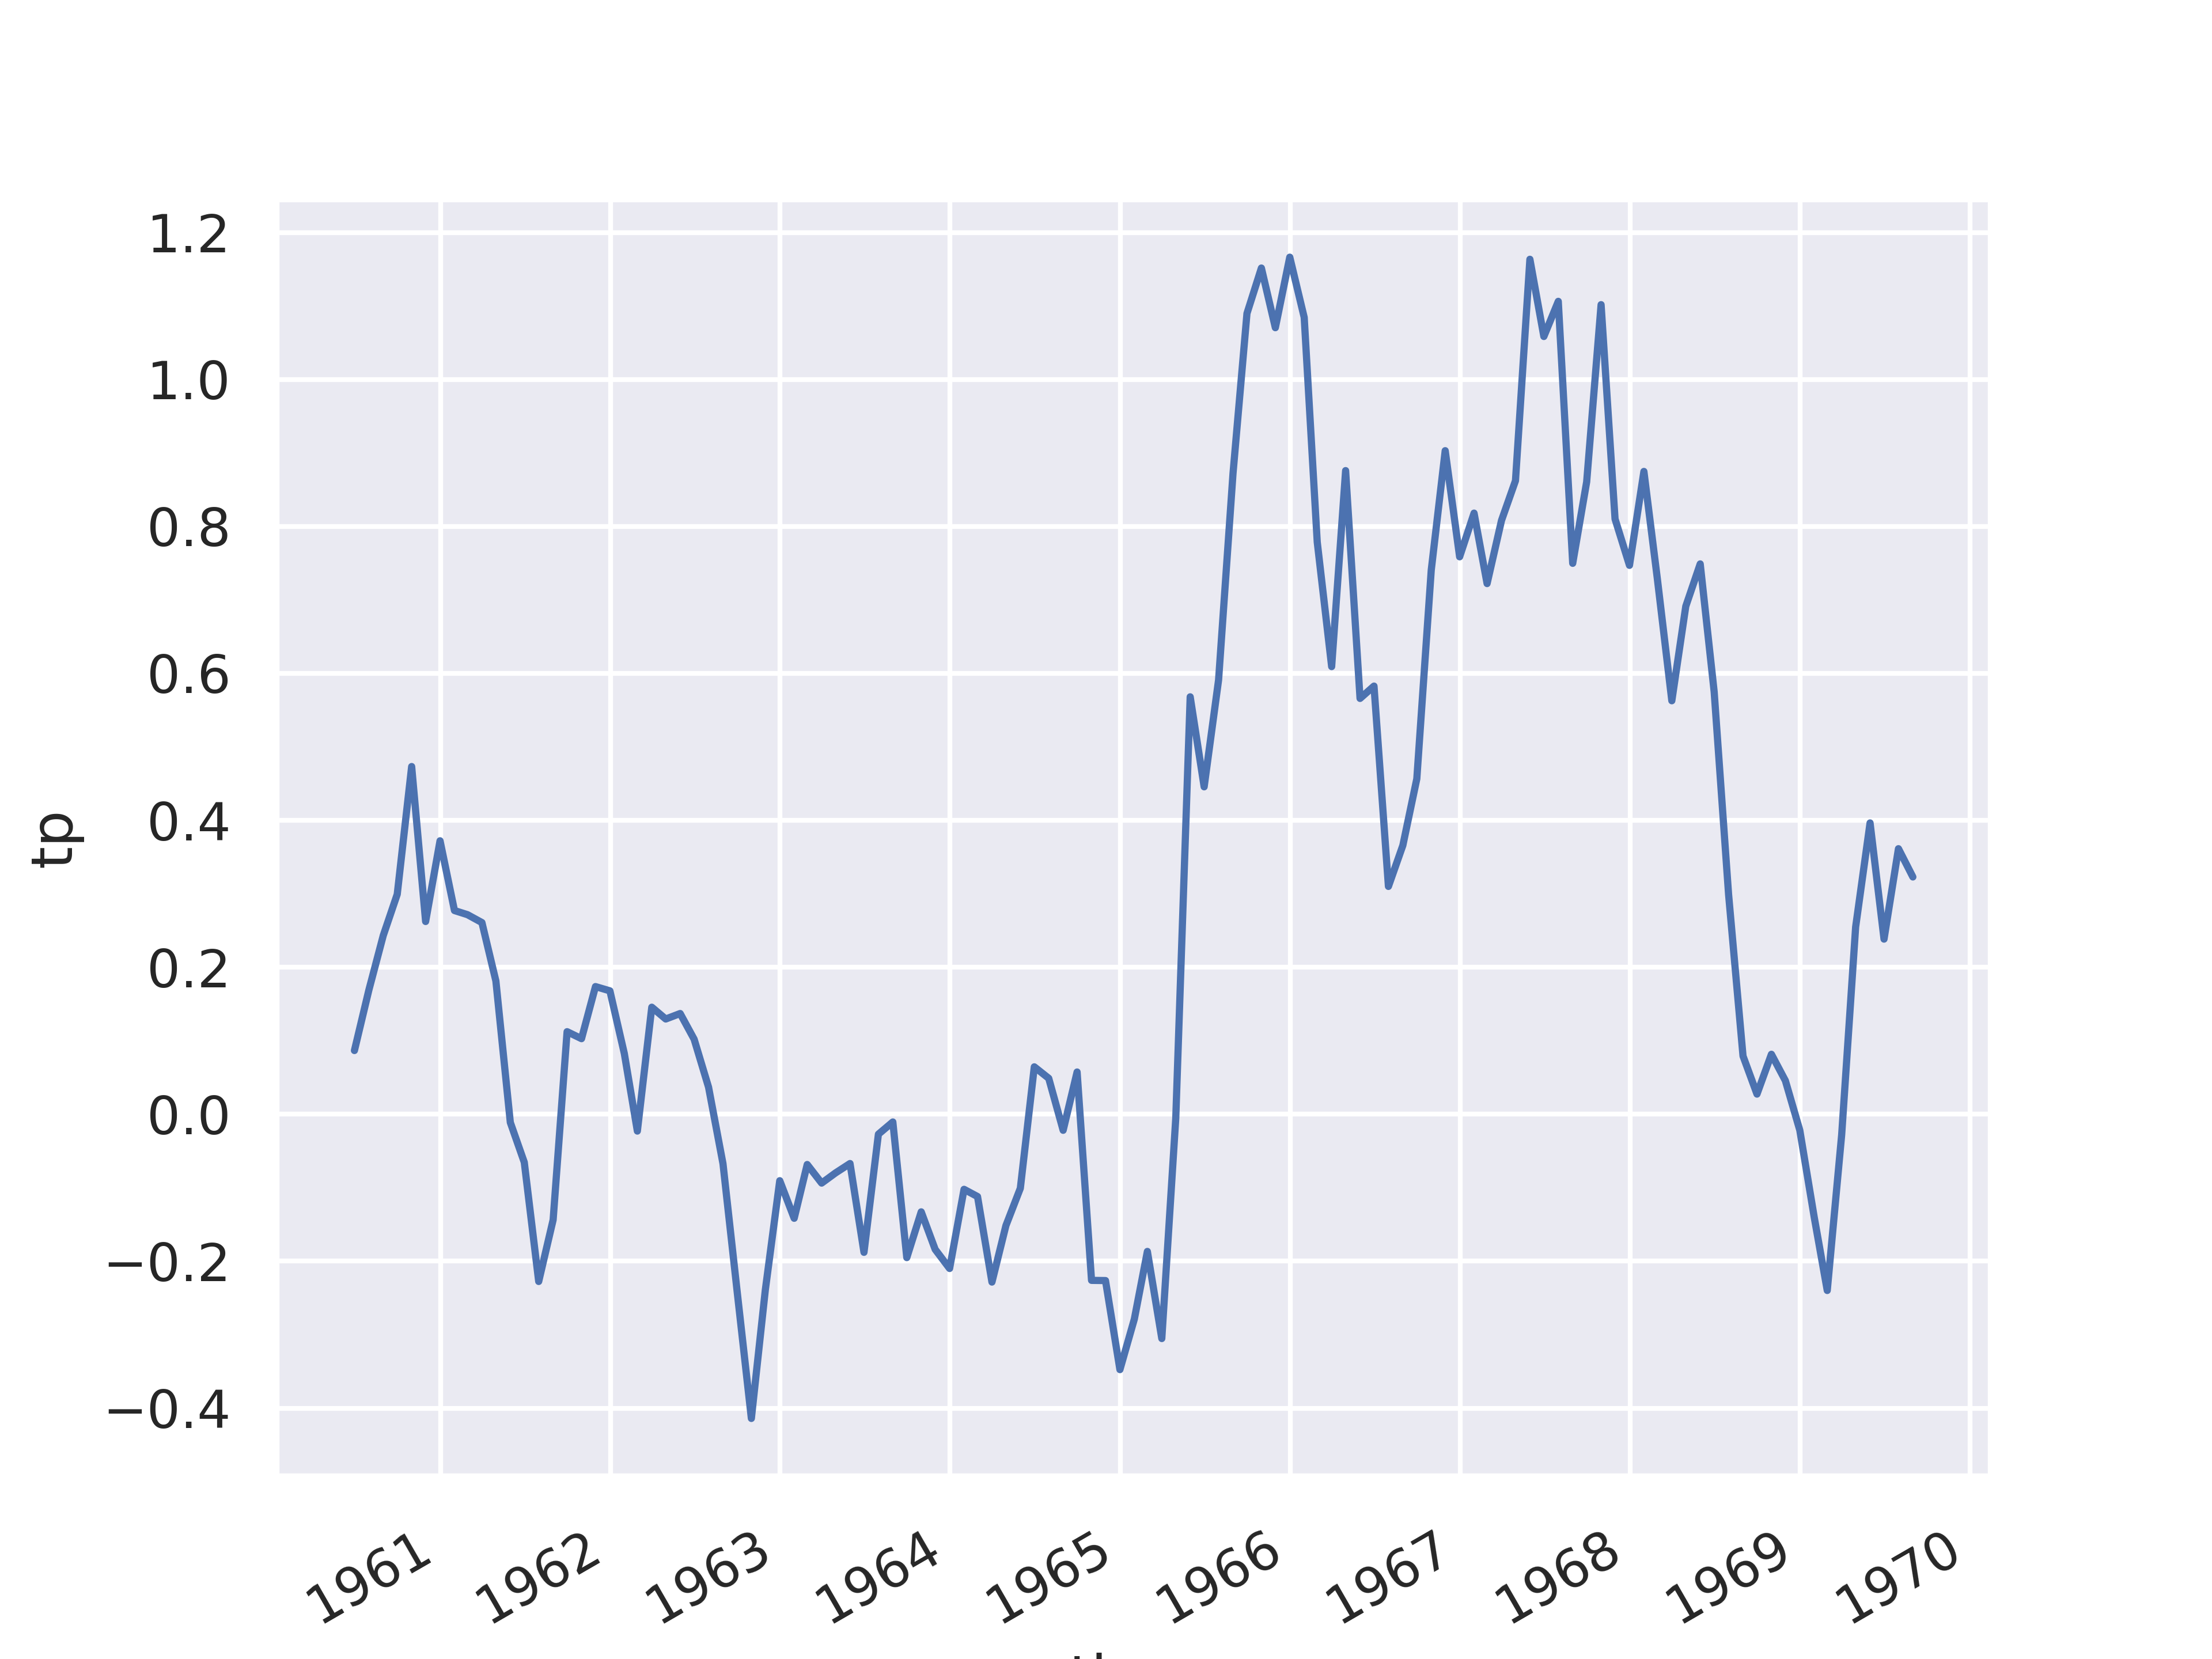
\includegraphics[width=0.8\textwidth]{precipitation_example.png}
\caption{Maximum precipitation anomalies with a 10-month moving average}
\end{figure}

\subsection{Example 2: Analysis of Wind Data}

In this example, we use the wind component to analyze wind data and calculate the standardized wind exceedance frequency over a given period.

\begin{lstlisting}[language=Python]
val = wind_component.std_wind_exceedance_frequency(('1960-01-01', '1964-12-31'), True)
val.rolling(time=12, center=True).mean().plot()
\end{lstlisting}

This code calculates the frequency at which wind speeds exceed a certain threshold over the period from 1960 to 1964, and smooths the results with a 12-month moving average. The generated graph shows the wind trends.

\begin{figure}[htbp]
\centering
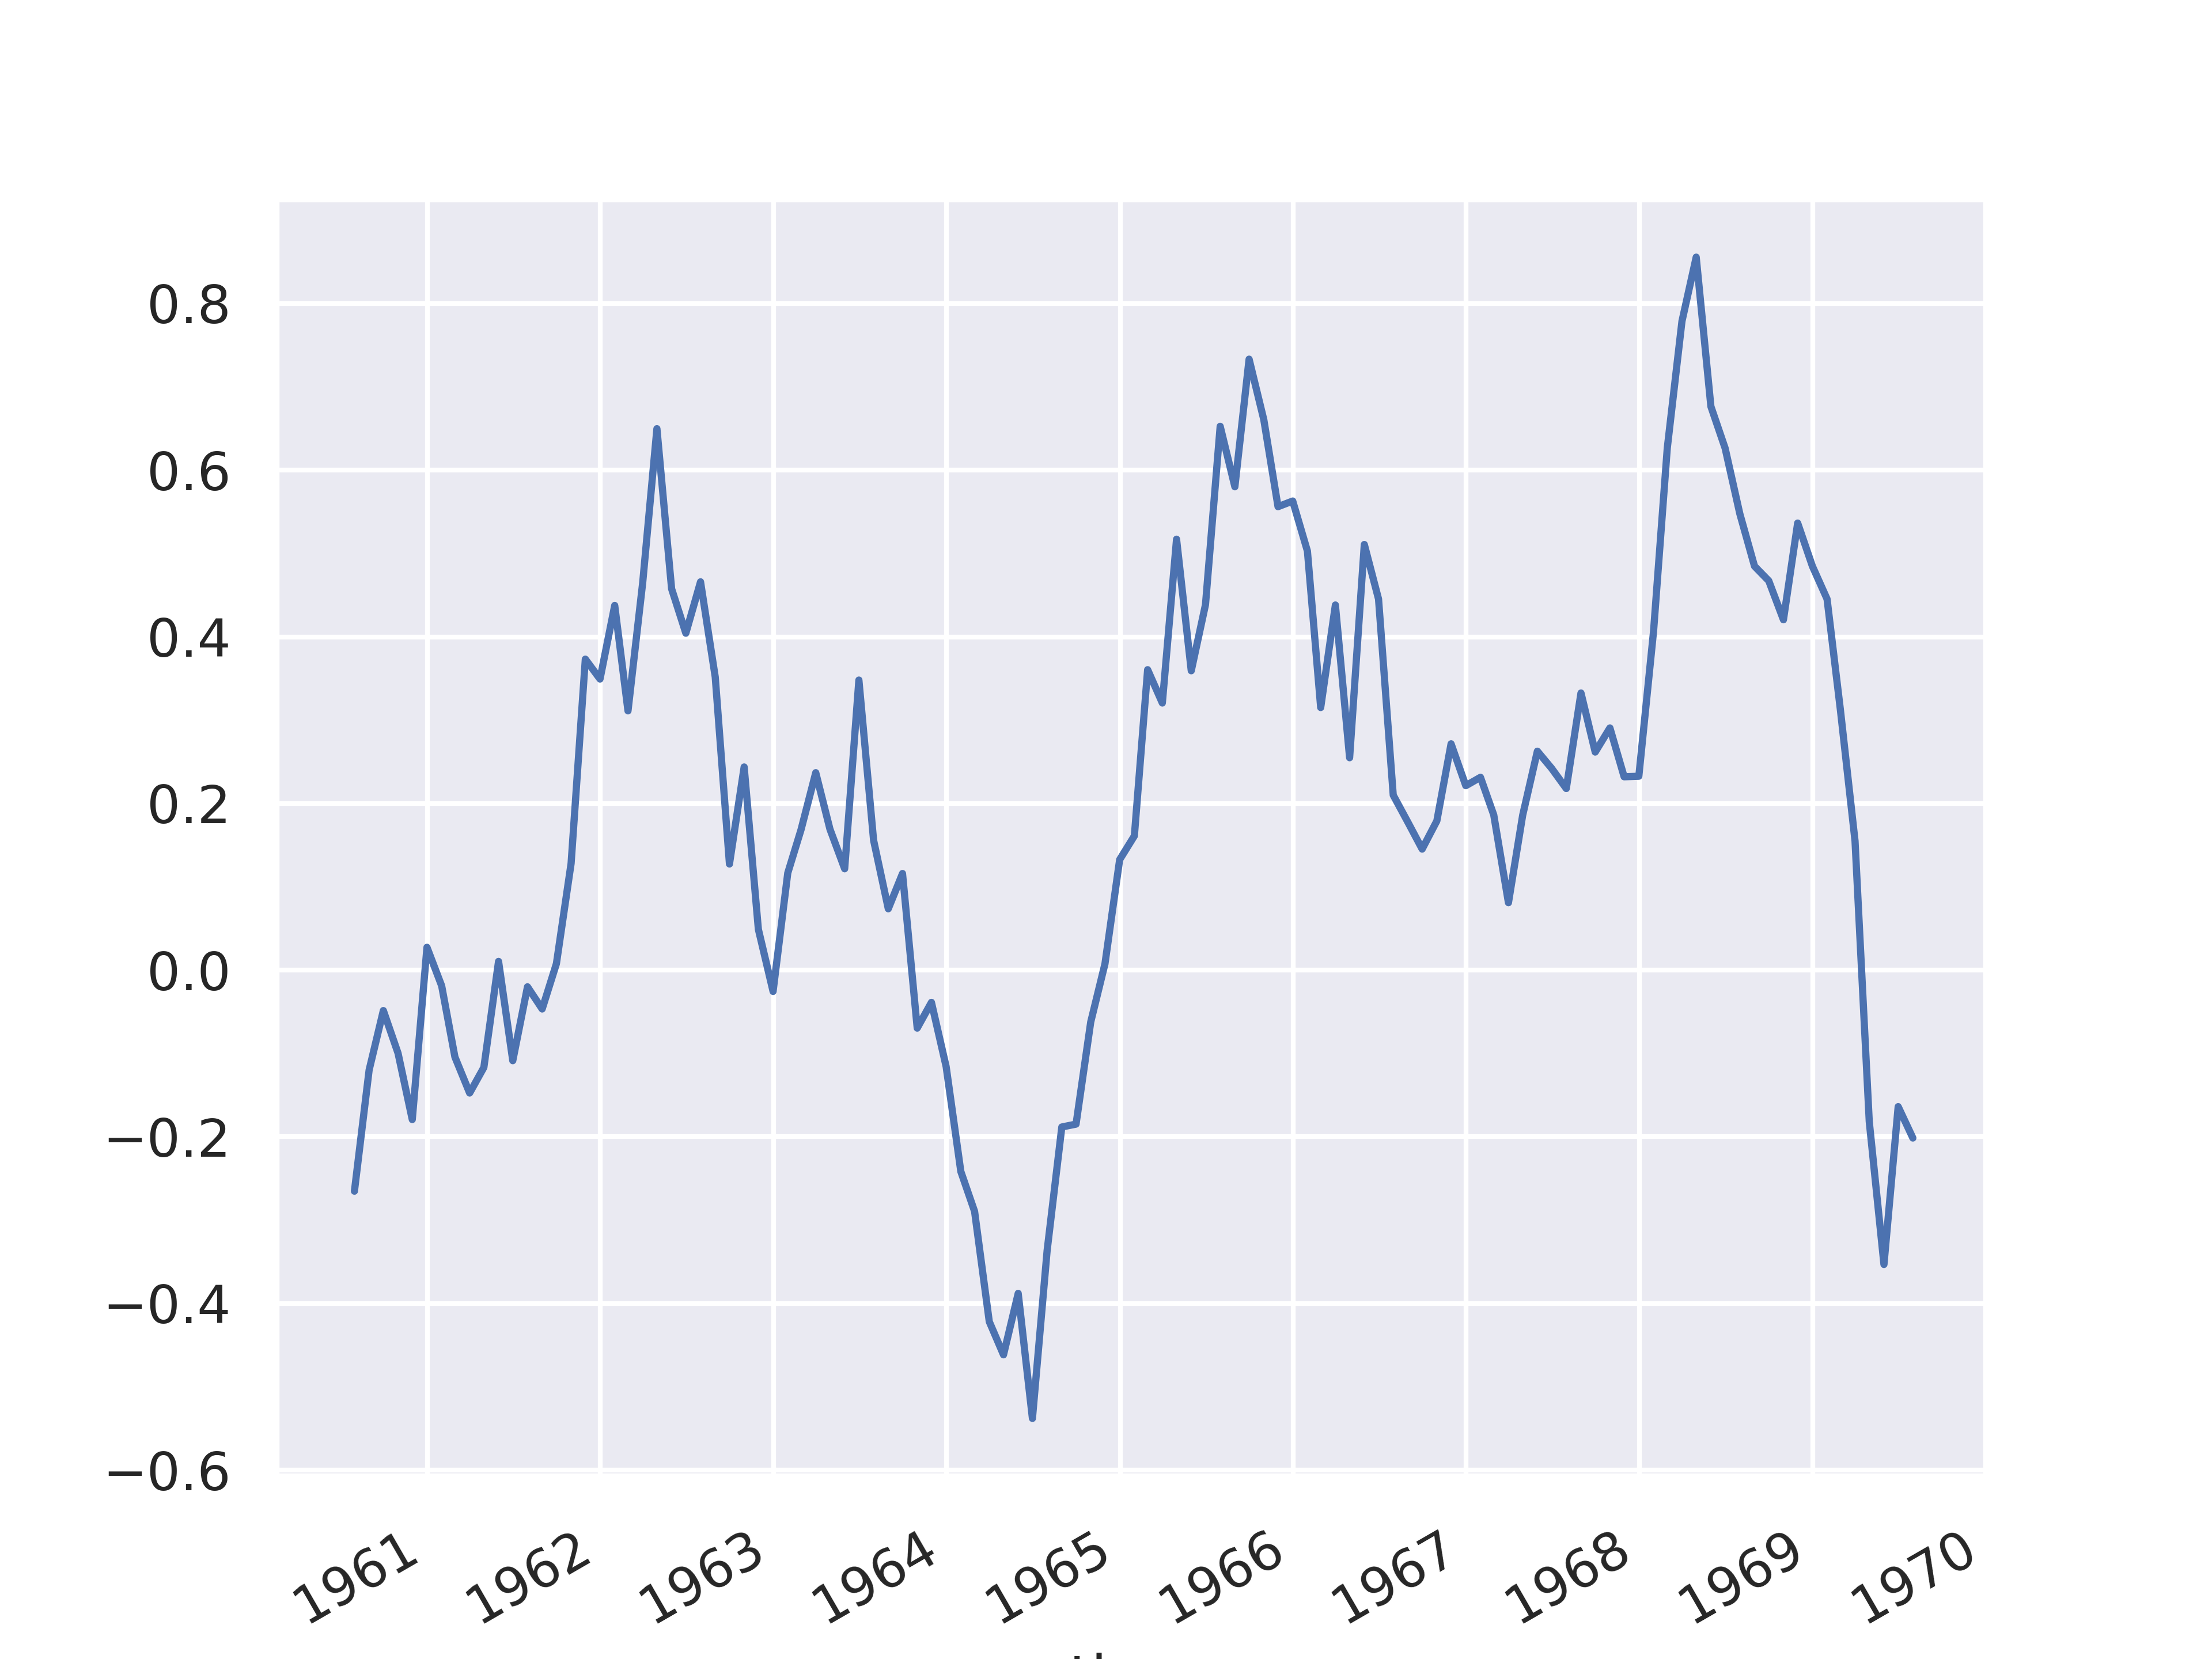
\includegraphics[width=0.8\textwidth]{wind_example.png}
\caption{Wind exceedance frequency with a 12-month moving average}
\end{figure}

\subsection{Example 3: Analysis of Drought Data}

This third example illustrates the use of the drought component to analyze drought periods, particularly consecutive days without precipitation.

\begin{lstlisting}[language=Python]
val = drought_component.std_max_consecutive_dry_days(('1960-01-01', '1964-12-31'), True)
val.rolling(time=12, center=True).mean().plot()
\end{lstlisting}

The code above calculates the maximum number of consecutive dry days over a five-year period, with data smoothing by a 12-month moving average.

\begin{figure}[htbp]
\centering
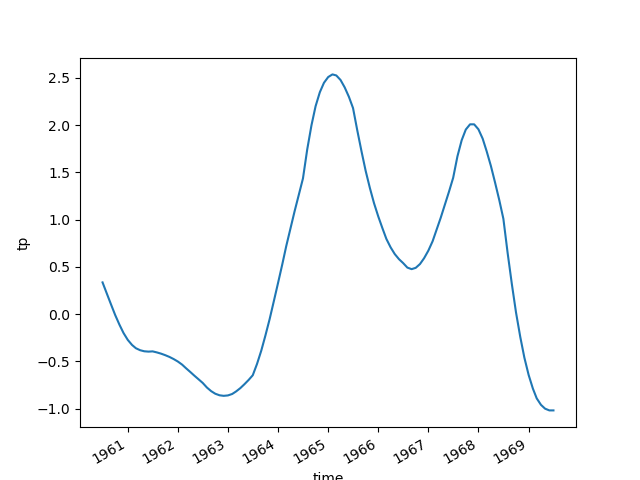
\includegraphics[width=0.8\textwidth]{drought_example.png}
\caption{Maximum consecutive dry days with a 12-month moving average}
\end{figure}

\subsection{Example 4: Analysis of Sea Level Data}

Finally, we show how to analyze sea level data using the corresponding component. This example highlights the average sea level evolution over a given period.

\begin{lstlisting}[language=Python]
a = niv_mer.mean(axis=1)
a.rolling(window=60, min_periods=12, center=True).mean().plot()
\end{lstlisting}

This code calculates the mean sea level and applies smoothing with a 60-month moving average. The resulting graph shows the variations in sea level over time.

\begin{figure}[htbp]
\centering
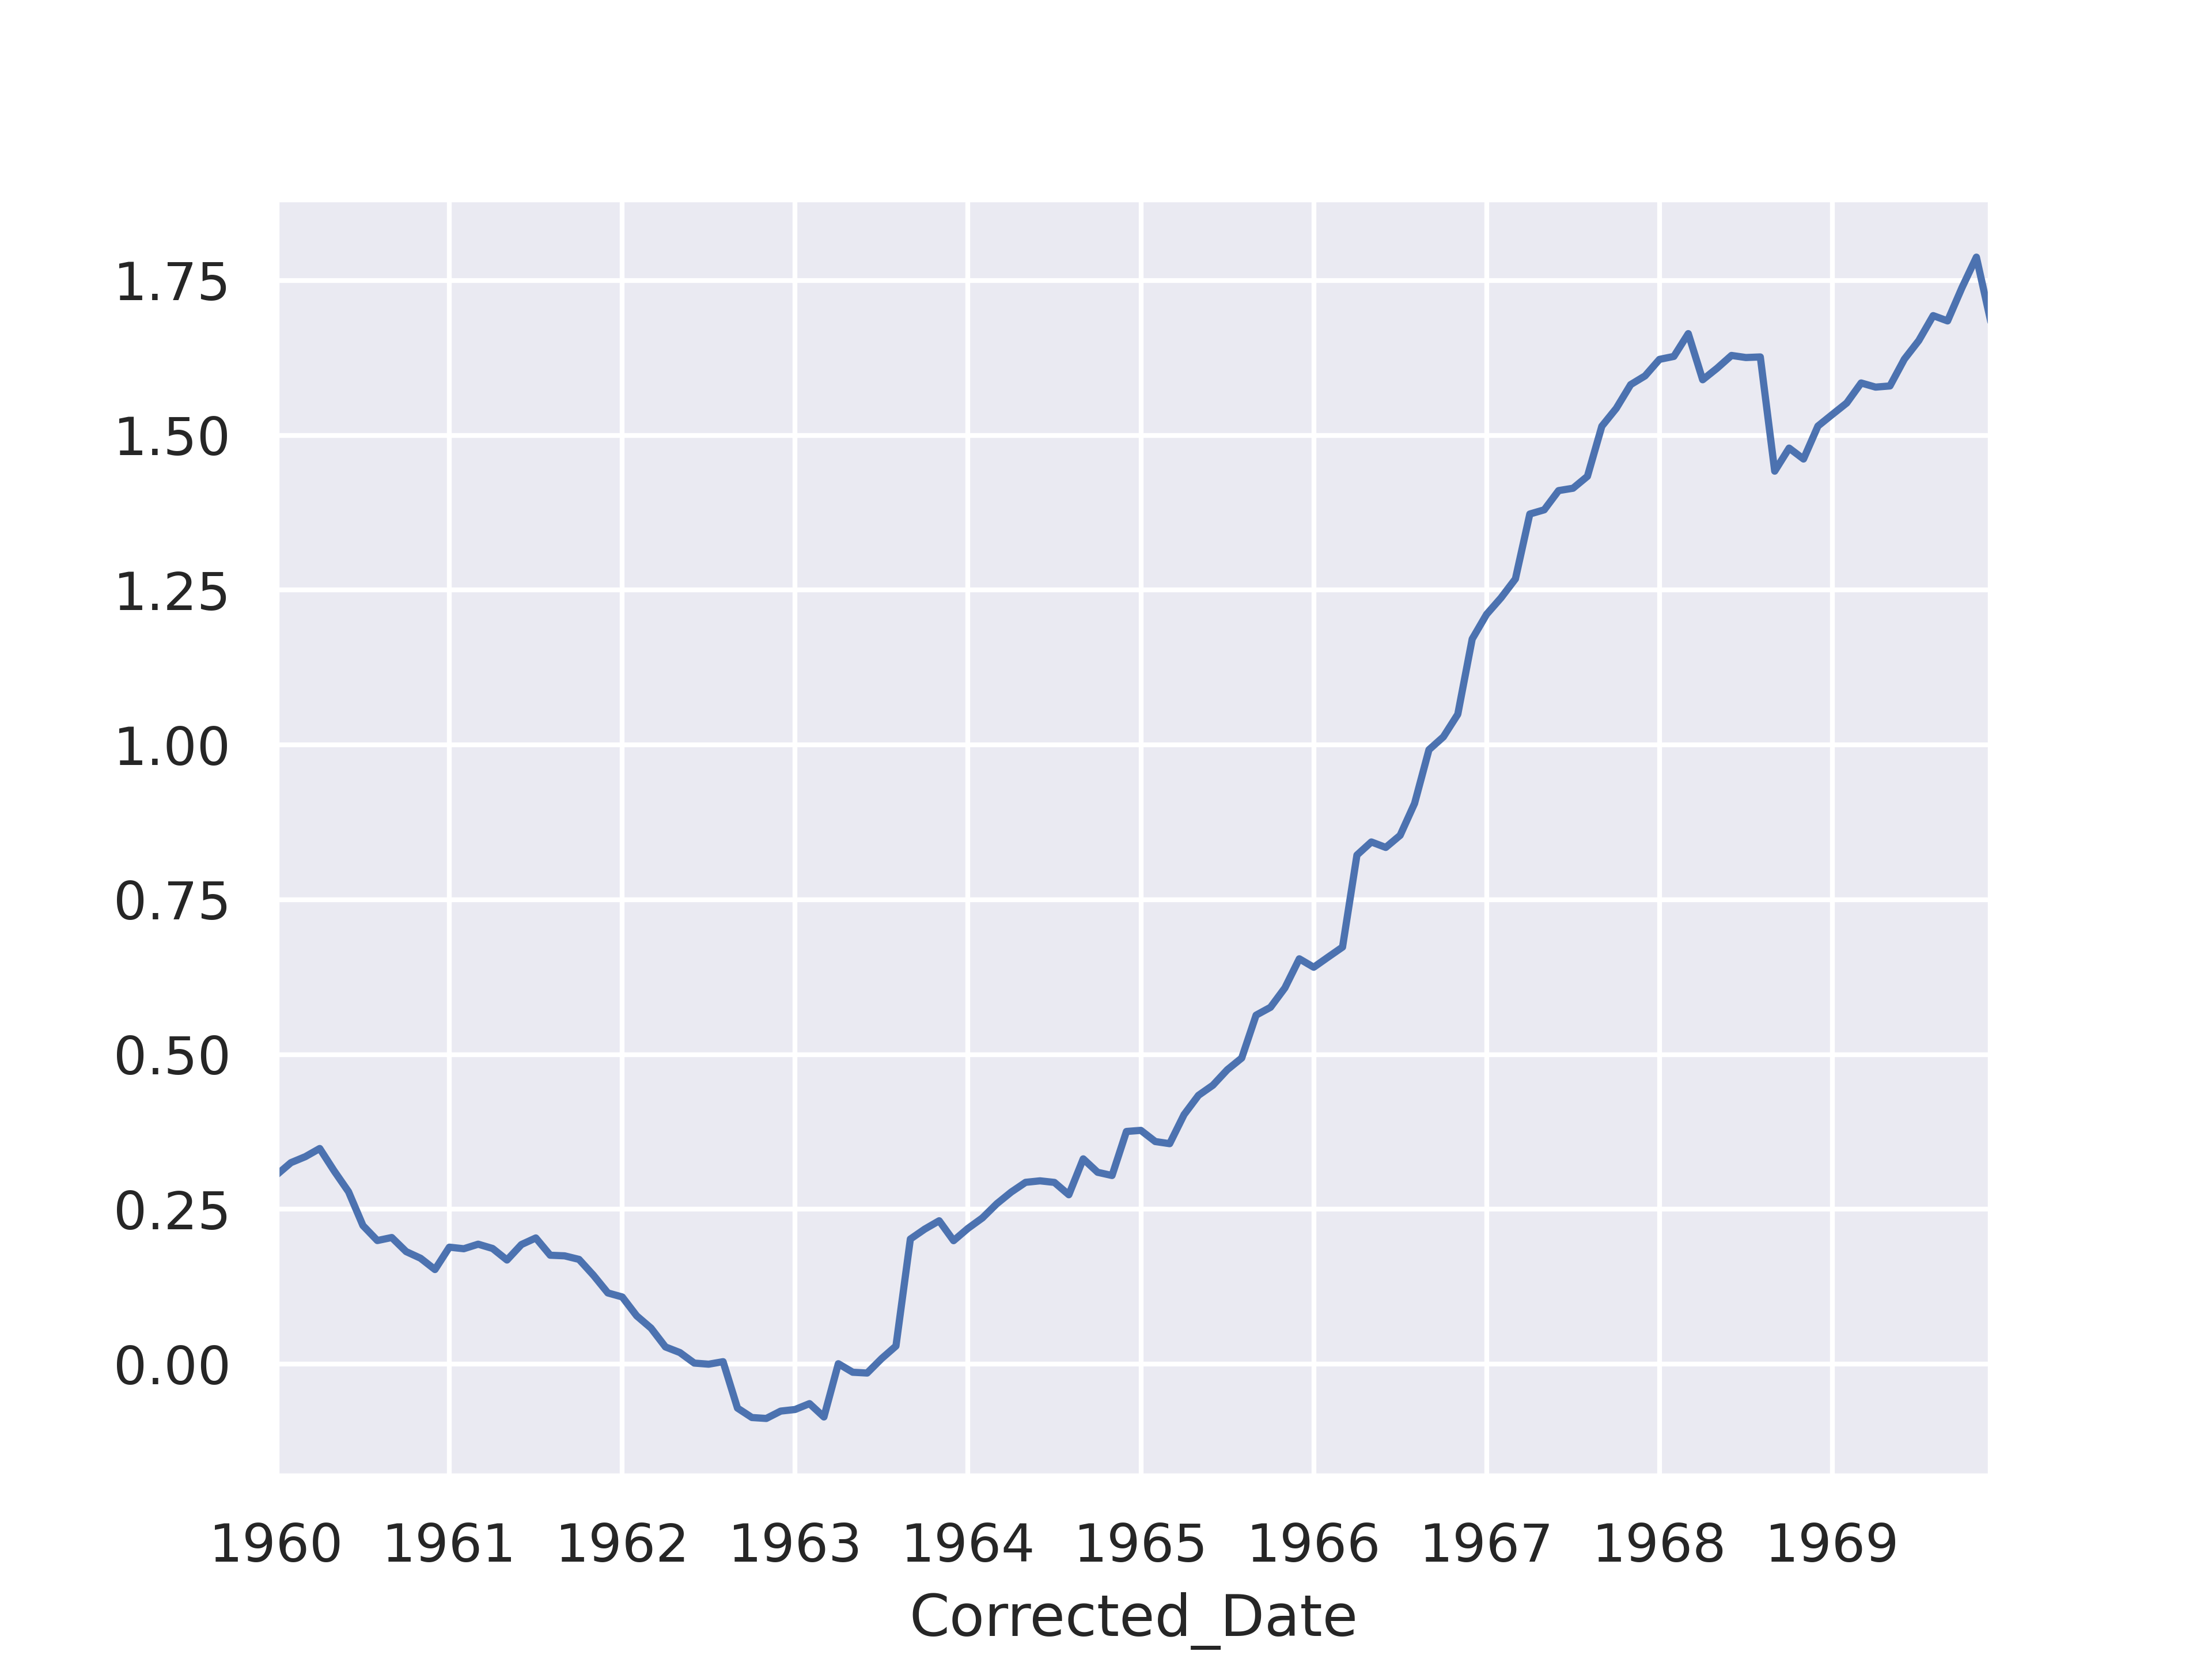
\includegraphics[width=0.8\textwidth]{sealevel_example.png}
\caption{Sea level evolution with a 60-month moving average}
\end{figure}

\subsection*{Conclusion}

These examples demonstrate how to use the developed components to analyze different aspects of climate data, using analysis techniques such as maximum anomalies, exceedance frequencies, and moving averages. Each component can be adapted to specific periods or other types of data depending on the needs of the analysis.

\section{Best Practices}
\label{sec:best-practices}
Recommendations for effective use of the project, resource management, etc.

\section{Troubleshooting and FAQ}
\label{sec:faq}
Solutions to common problems and answers to frequently asked questions.

\subsection{TypeError: \texttt{\_\_init\_\_()} got an unexpected keyword argument 'base'}
This error often occurs due to an incompatibility between specific versions of \texttt{xarray} and \texttt{pandas}. It might manifest when trying to resample data using xarray’s \texttt{resample()} function.

\paragraph{Cause:}
The error is usually caused by an incompatibility between the installed versions of \texttt{xarray} and \texttt{numpy}. Certain versions of \texttt{xarray} expect specific parameters in the underlying \texttt{pandas} and \texttt{numpy} functions, which may have changed or been deprecated in newer versions.

\paragraph{Solution:}
A potential solution is to uninstall the current version of \texttt{numpy} and let \texttt{xarray} install the compatible version:

\begin{lstlisting}[language=bash]
pip uninstall numpy
pip install xarray
\end{lstlisting}

This approach allows \texttt{xarray} to handle the installation of a compatible version of \texttt{numpy}, resolving the mismatch. After this, try rerunning your script to see if the issue is resolved.

\paragraph{Alternative Solution:}
If the above solution does not work, consider explicitly specifying compatible versions of \texttt{xarray} and \texttt{numpy} in your environment configuration, or using a pre-configured \texttt{conda} environment as described in the installation section.

\subsection{Other common issues}
\textbf{Error: Permission denied when connecting to \texttt{libvirt-sock}} \\
This issue often arises due to insufficient permissions to access the \texttt{libvirt} daemon. Ensure your user is part of the \texttt{libvirt} group and that you have restarted your session after adding your user to the group.

\subsection{FAQ}
\begin{itemize}
    \item \textbf{How do I update dependencies safely?} \\
    Use \texttt{conda} environments or virtual environments to manage dependencies, which allows you to update or downgrade specific packages without affecting your system-wide Python installation.

    \item \textbf{Why do I get a performance warning in \texttt{xarray}?} \\
    Performance warnings typically indicate operations that are non-optimal, such as unchunked Dask arrays or large in-memory computations. Review your Dask setup and consider optimizing your chunk sizes or using Dask more effectively.
\end{itemize}

\section{Conclusion}
\label{sec:conclusion}
Summary and future prospects.

\end{document}
